\documentclass[10pt, a4paper, twocolumn]{article}
\usepackage[utf8]{inputenc}
\usepackage[T1]{fontenc}
\usepackage{graphicx}
\usepackage{beton}
\usepackage{eulervm}
\usepackage{amsmath}
\usepackage{bm}
\usepackage{microtype}
\usepackage[medium, compact]{titlesec}
%\usepackage[inline]{asymptote}
%\usepackage{tikz-cd}
\DeclareFontSeriesDefault[rm]{bf}{sbc}
% \usepackage{amssymb}
%% Turing grid is 21 columns (of 1cm if we are using A4)
%% Usually 4 "big columns", each of 4 text cols plus 1 gutter col;
%% plus an additional gutter on the left.
\usepackage[left=1cm, right=1cm]{geometry}
%\usepackage[Ragged, size=footnote, shape=up]{sidenotesplus}
\setlength{\columnsep}{1cm}
\title{Blockworld physics}
\author{}
\date{\today}

\begin{document}
\maketitle

\section{Earth blocks}

\subsection{General overview}

The challenge with Earth blocks is to model the hydrology: the
movement of water through the blocks.

Each Earth block contains some water. Water can move from block to
block. In real life, there are (I think!) two main processes: (1)
groundwater, which flows like a viscous fluid through saturated rock;
(2) moisture, which is transported via a diffusion-like process
(capilliary action, possibly?) in unsaturated rock.

Water tends to move:
\begin{itemize}
\item down, under gravity; 
\item from blocks with high pressure to blocks with low pressure; 
\item from blocks with high water content to blocks with low water
  content.
\end{itemize}

The following is a version of all of this. I am not claiming physical
realism with the real world but it is “physically plausible.”

\subsection{Block parameters}

All parameters are integers unless otherwise stated. An Earth block
has a single parameters, the water content, $w$.

The hydrostatic pressure, $p$, is then dervied from the water
content. See figure~\ref{fig:pressure} for the relationship between
the two.
\begin{figure}[ht]
  \centering
  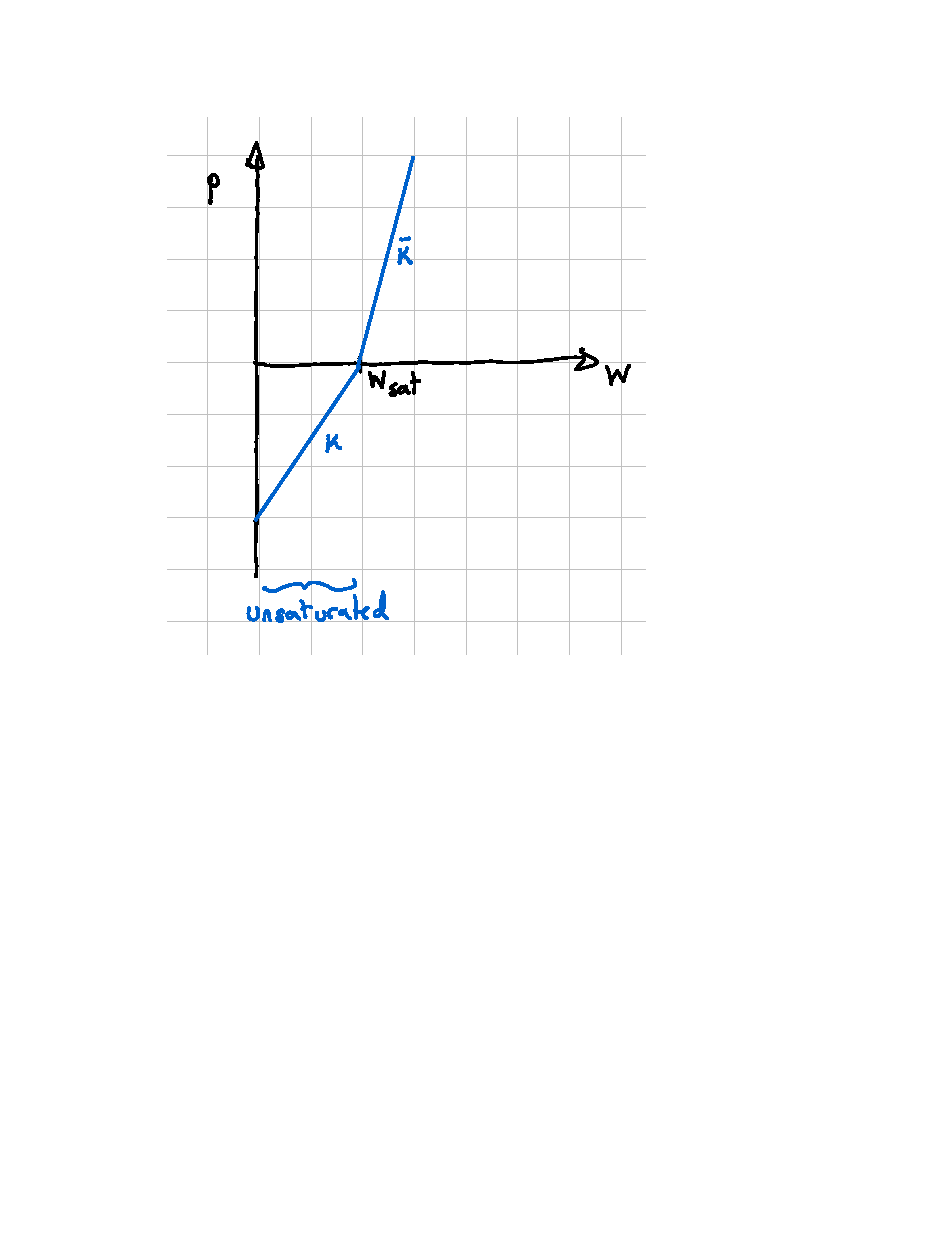
\includegraphics{fig-pressure.pdf}
  \caption{Dependence of hydraulic pressure on Earth block water
    content. Note that the pressure of an unsaturated block is
    effectively negative.}
  \label{fig:pressure}
\end{figure}

The units of pressure are length. A pressure of $1$ is the weight of
$1$ unit of water acting on an area of one block face. (Note that if
we had pure Water blocks, they would not necessarily be 1 unit of
water.)

\subsection{Global constants}

The following are the ``constants of nature.'' Their meaning is given
roughly here but the real meaning of these terms is just how they
enter into the equations of state.

\begin{enumerate}
\item Saturation level $w_{\text{sat}}$ (integer): the maximum water
  content per block.
\item Permeability, $\sigma$: the inverse of the number of world ticks over
  which one unit of water flows between blocks subject to a pressure
  gradient of~$1$.
\item Compressibilit, $\kappa$ (in unsaturated regime), $\bar{\kappa}$ (in
  saturated regime). The marginal increase in pressure for one unit
  increase in water water content; that is $\Delta p/\Delta w$. 
\item Gravitational constant is chosen to make the weight of 1 unit of
  water equal to~1.
\end{enumerate}
  
\subsection{Equations of motion}

This is a two-step algorithm. We start with the water content, $w$, of
each Earth block. The hydraulic pressure, $p$, of each block, is then
a piecewise linear function of~$w$, as described above.

\begin{enumerate}
\item Compute the water flux across each face.
  \begin{enumerate}
  \item For each face, compute the ``pressure gradient'' as the
    difference in $p$ between the two blocks separated by this
    face. In addition, if the face is a lower face, add a force that
    is the water content of the block above. (This is a gravitational
    term.)

  \item For each face, compute the \emph{preliminary flux} across that
    face is the pressure gradient times the permeability.

  \item Now potentially make adjustments to the fluxes. For each cell,
    consider all outgoing preliminary fluxes. We adjust these fluxes
    by ``giving $w$ to them in order from largest to smallest, until
    $w$ runs out,'' as follows. If the total outgoing preliminary flux
    is less that $w$, make no adjustment to the preliminary
    fluxes. Otherwise, start by assigning $w$ to the largest
    preliminary flux. If $w$ is less than the flux, adjust that flux
    to $w$ and the remaining fluxes to zero. Otherwise make no
    adjustment to the largest flux, subtract the largest flux from
    $w$, and continue with the next largest flux. Continue until there
    is no more water left.
  \end{enumerate}

\item For each cell, adjust its water content by the sum of the
  fluxes.
\end{enumerate}

\subsection{Boundary conditions}\label{sec:boundary}

Some Earth blocks abut other blocks. If the face is adjacent to Air,
treat it as an empty block with pressure zero. (At the moment, water
exiting into Air will be lost, but won't in fact happen very often.)

If the face is adjacent to Rock, treat the pressure gradient as zero
(so that there is no flux across this face).

\subsection{Back of the envelope estimates}

\subsubsection{Diffusion timescale}

$\delta_t M \sim \sigma \kappa \nabla^2 M$. So ... $\sigma\kappa$ has dimensions $T^2 L^{-1}$.  

We should probably have $\kappa\sigma < 1 $, say $1/8$? With $\kappa~1$.

\subsubsection{Gravity}

What water content is just balanced on top of a just-saturated block?
The ``gravitational pressure'' is $w$; whereas the upward pressure
difference is $\kappa(w_\text{sat} - w)$. These balance when $w = \kappa
w_\text{sat} / (1+\kappa)$. 



\section{Light}

Light is a parameter of Air blocks. Light is $L_{\text{sky}}$ in any
block with unobstructed vertical line of sight to the sky; otherwise
it is $L_{\text{amb}}$. (Maybe we'll implement some radiosity model
later.)

\section{Plant}

A Plant block has two main components: the ``physical'' plant (which
follows ``physical laws'') and the controlling state machine. This
section describes the physical component.

The dynamic parameters of a Plant block are:
\begin{enumerate}
\item An identifier of this plant's species;
\item (Possibly) an opaque identifier of ``this plant;'' 
\item Water content (just like Earth blocks);
\item Energy content (another integer). An energy of $1\,\textrm{e}$ is the energy
  required to lift unit water by one block;
\item For each face, a permeability. (Note that there are two
  permeabiliities for each face, one for each block on either side.)
\end{enumerate}

The static parameters are:
\begin{enumerate}
\item Saturation level (as Earth blocks, but probably higher);
\item Compressibilities (saturated and unsaturated, like Earth
  blocks);
\item $F_{\text{max}}$, the maximum force a plant block can apply
  across a face to water.
\item The maximum permeability of a face, $\sigma$.
\end{enumerate}

\subsection{Plant actions}

Every state-machine tick, the Plant block can choose any number
(including all) of the
following actions:

\begin{enumerate}
\item For each face (including faces exposed to air), set the
  permeability from zero up to a maximum $\sigma$.
\item For each open face apply a ``pumping force'' up to a maximum of
  $F_{\text{max}}$.
\item Transmit arbitrary energy to any adjacent plant block. (This
  action takes place before any other actions.) The energy thus
  transferred may not leave the block with negative energy. Energy is
  transferred in order of instructions.
\item Post a ``signal'' on any face. (Data format to be determined.)
\end{enumerate}

\subsection{Plant sensors}

The plant state-machine has available to it the following data:
\begin{enumerate}
\item The face that is ``up.'' 
\item The energy in this block.
\item The water content in this block.
\item The outcome permeability of each side.
\item The nature of each adjacent block (plant, air, earth, other);
\item The water pressure in adjacent blocks.
\item The signal posted by the adjacent block.
\end{enumerate}

\subsection{Plant dynamics}

\subsubsection{Pumping}

\begin{enumerate}
\item For each block, compute pressure in the usual way. However, the
  pressure/density relation is different: see
  figure~\ref{fig:plant-pressure}.
\item For each face, compute the total force across this face, as the
  sum of:
  \begin{itemize}
  \item the pressure difference;
  \item the two pumping forces (one from each adjacent block);
  \item the gravitational term.
  \end{itemize}
  Except that, if this block's energy is zero or negative, no pumping
  can be done (the pumping force is set to zero).
\item For each face, compute the resultant permeability as being the
  ``parallel sum'' of the two permeabilities set by the adjacent
  blocks. (The inverse of the resultant is the sum of the inverses.)
  For the purpose of this calculation, Air has infinite permeability;
  Rock has zero permeability.
\item For each face, compute the resultant force.
\item From the resultant force and the permeability, compute the net
  preliminary flux.
\item Next, adjust the preliminary fluxes (as before) to ensure that the outflow
  does not make the volume negative.
\item Then, for each pump, compute the energy consumption as the force
  \emph{of that pump} multiplied by the flux in the direction of the
  pump. (If the flux is opposite the pumping direction, no energy is
  consumed.)
\item Subtract the total energy consumption from the block's
  energy. (It is allowed to go below zero, but no pumping can then
  take place until it is brought above zero.)
\end{enumerate}

\begin{figure}[ht]
  \centering
  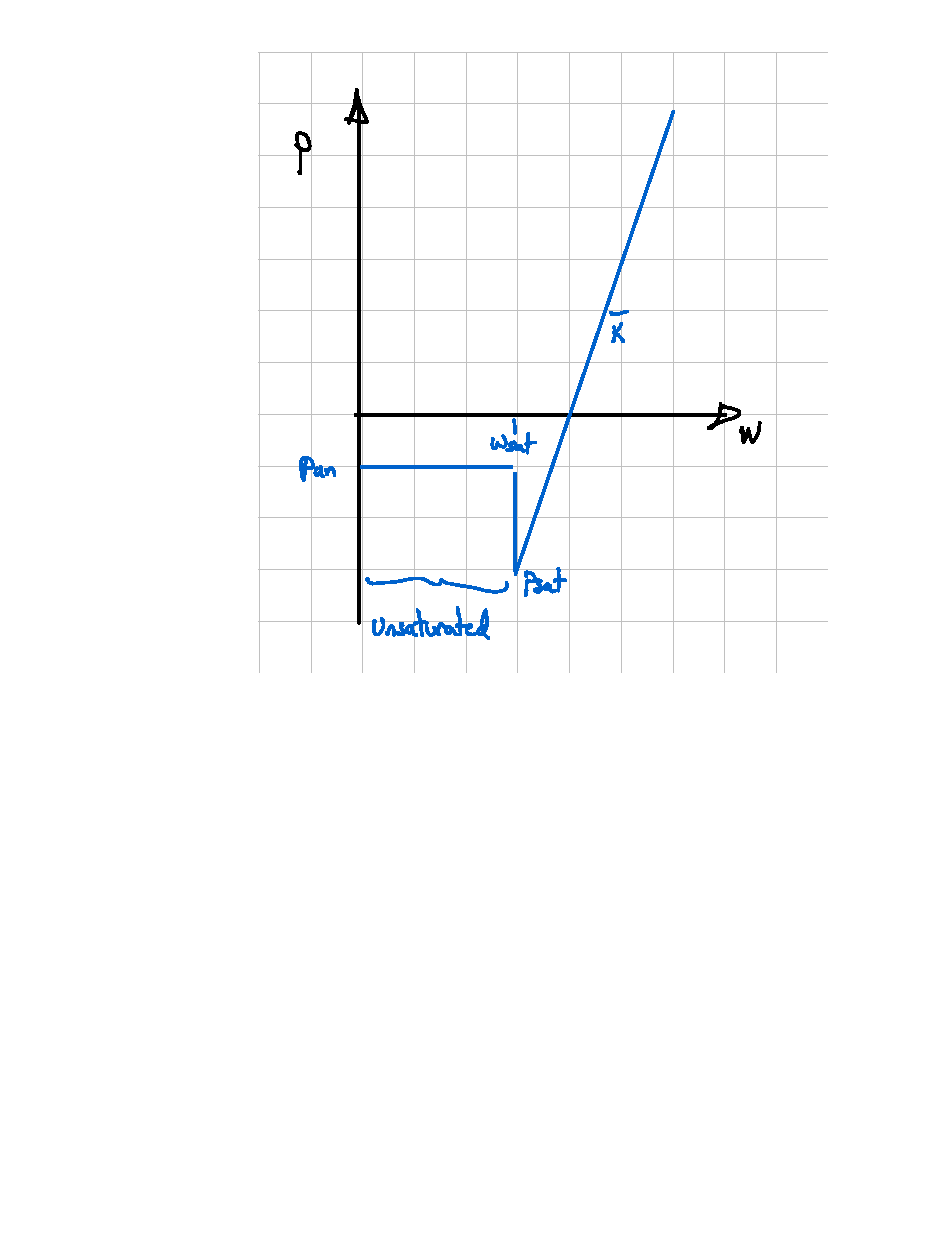
\includegraphics{fig-plant-pressure.pdf}
  \caption{Dependence of hydraulic pressure on water content for Plant
    blocks. The pressure is constant and negative up to the saturated
    limit (this lets the roots ``suck in'' water), then jumps to being
    more negative and incompressible. The idea for this jump is to
    allow water to be ``pulled upwards'' as it evaporates from the
    higher blocks, at least up to some point when the connection
    ``breaks.''}
  \label{fig:plant-pressure}
\end{figure}

  
  
\subsubsection{Evaporation}

\subsubsection{Photosynthesis}

  




\section{Wacky ideas section}

\begin{itemize}
\item It takes energy to change the direction and strength of the face
  pumps. 
\item Generators (like pumps, but in reverse).
\end{itemize}


\end{document}
